\section{Evaluation}
\label{sec:evaluation}

This section evaluates \minotaur{}.


\subsection{Correctness}

Every optimization discovered by \minotaur{} has been formally verified by
Alive2.
%
Even so, bugs might remain in the instruction semantics that we have
added to Alive2, in our cut extractor, in our rewrite mechanism, or in
Alive2 itself.
%
To defend against implementation errors, we have compiled numerous
open source applications using \minotaur, and then run those applications'
test suites, to ensure that they were not miscompiled.
%
Furthermore, we have compiled SPEC CPU 2017 using \minotaur{} and
used the SPEC drivers to ensure that all of its benchmarks behave
as expected.


\subsection{Effect of Depth Bounds in the Cut Extractor}
\label{sec:loops}

%1345 loops are integer only + vectorizable
%plot only shows 879 loops, these are the loops touched by minotaur.

% 2386 loops are integer / fp + vectorizable
% depthlimit 5: 26339 exprs (305 opt), 290 source changed, 667 min elapsed
% depthlimit 4; 24334 exprs

% \begin{figure*}[tbp]
%   \centering
%   \subfloat[Targeting Intel Cascade Lake; geomean=1.061x\label{plot:loops-intel}]{
%     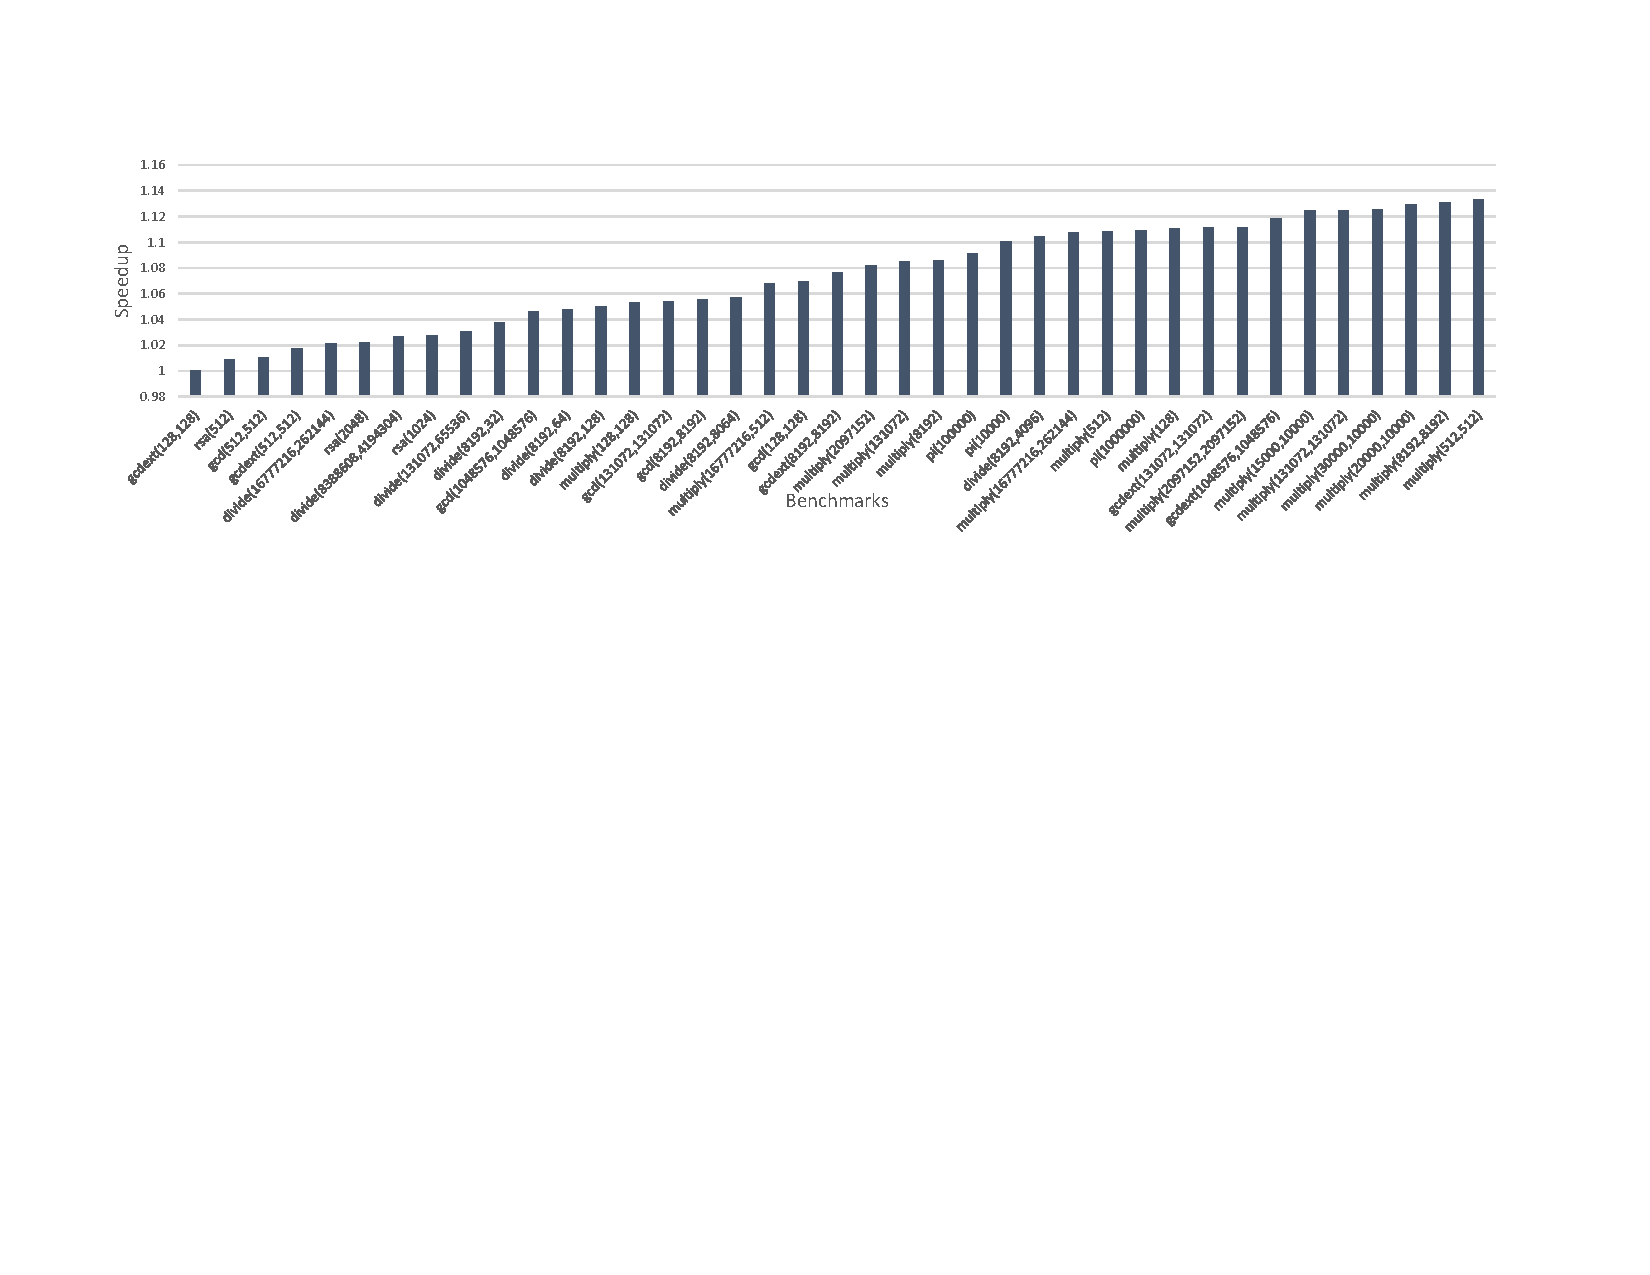
\includegraphics[page=1,width=\linewidth]{figures/data.pdf}
%   }`
%   \hfill'
%   \subfloat[Targeting AMD Zen 3; geomean=1.021x\label{plot:loops-amd}]{
%     \includegraphics[page=2,width=\linewidth]{figures/data.pdf}
%   }
%   \caption{Speedups---estimated by LLVM-MCA---due to running \minotaur{}
%     on a loop micro-benchmark suite}
% \end{figure*}

It is important for \minotaur{} to extract cuts that are of an appropriate
size.
%
If they are too large, compile times suffer and also the SMT solver
can be overwhelmed, leading to timeouts; if cuts are too small, then
they form an insufficient basis for driving an optimization.
%
To determine a good value for $B$, the depth parameter to the cut
extraction procedure shown in Algorithm~\ref{alg:slicing}, we
performed an empirical study.
%
We started with FlexC's benchmark suite~\cite{woodruff2023rewriting},
a collection of 2,386 compilable, non-trivial C functions containing
loops from FFMPEG, FreeImage, DarkNet, xz, bzip2, and the LivermoreC
benchmark.
% \footnote{The loop data set was provided
% by Alexander Brauckmann and Michael O'Boyle at the University of
% Edinburgh, UK\@.  At present, no citable reference for this work
% exists.}
%
When compiled to LLVM IR, these functions contain a total of 123,062
instructions; thus, our cut extractor was invoked 123,062 times for
each depth bound.
%
We chose this code as the basis for our experiment because it is
derived from real applications while also being small enough to
keep compile times manageable (compared to, e.g., SPEC CPU 2017,
which is much larger).


\begin{figure}[tbp]
  \centering
  \subfloat[Unique cuts extracted\label{fig:loop-expression}]{
    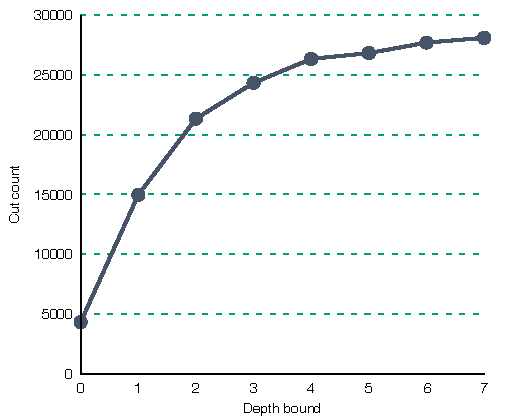
\includegraphics[width=0.32\linewidth]{figures/spec/expression-count.pdf}
  }
  \hfill
  \subfloat[Unique opts. synthesized\label{fig:loop-optimization}]{
    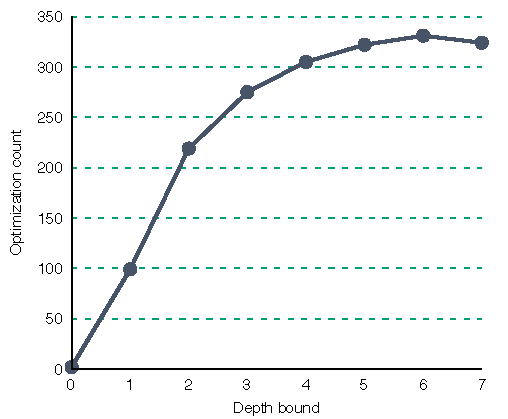
\includegraphics[width=0.32\linewidth]{figures/spec/optimization-count.pdf}
  }
  \hfill
  \subfloat[Compilation time\label{fig:loop-buildtime}]{
    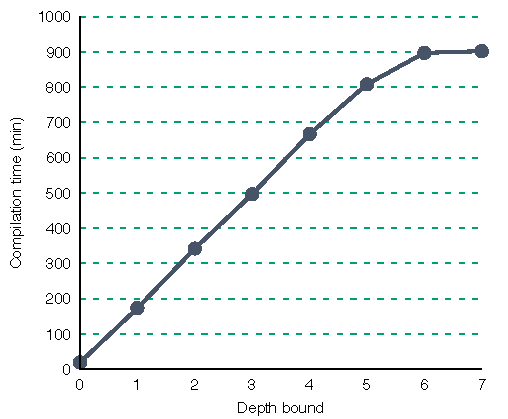
\includegraphics[width=0.32\linewidth]{figures/spec/compilation-time.pdf}
  }
  \caption{Evaluating the effect of varying $B$, the depth bound for
    cut extraction}
  \label{fig:loop}
\end{figure}


We then ran \minotaur{} on these functions with all depth bounds from
0--7, measuring the number of unique cuts that were extracted, the
number of optimizations found, and the compilation time.
%
We used a one-minute timeout for individual Z3 queries, and we also
gave \minotaur{} a total of up to five minutes to synthesize an optimized
version of each cut.
%
Figure~\ref{fig:loop} summarizes the results of this experiment.
%
The number of unique cuts that are extracted grows quickly with $B$,
but eventually begins to saturate simply because the functions being
compiled do not always have very long dependency chains.
%
The number of synthesized optimizations also grows quickly, but it
peaks when $B=6$ and then it decreases because the size of the cuts
causes many solver timeouts.
%
Finally, the total compile time increases smoothly with the depth
bound, eventually leveling off as most solver queries time out.


For the experiments in the rest of the evaluation section, we chose
$B=4$ because this gets pretty close to the maximum observed number of
optimizations without requiring exorbitant compile times.
%
It seems likely that there is room for improvement in this aspect of
\minotaur: perhaps the depth bound should be determined adaptively.
%
In this scenario, we would extract more and more components into the
cut, until either an optimization is found or else the solver begins
to time out.
%
We leave explorations of this nature for future work.


\subsection{Speedups for Benchmarks and Applications}

In this section, we show how \minotaur{} speeds up real-world benchmarks
and applications.

\paragraph{Experimental setup}
%
We used two machines for our evaluation: one with an Intel Xeon Gold
6210U processor running at 2.5\,GHz (this implements the Cascade Lake
microarchitecture~\cite{cascadelake}) and the other with an
AMD Ryzen 5950x processor
running at 3.4\,GHz (this implements the Zen~3 microarchitecture~\cite{zen3}).
The Intel machine supports the AVX-512 instruction set.
%
Both machines run Linux and were idle except for a single core running
our benchmarks.
%
To reduce the performance variation caused by frequency scaling, we
disabled turbo boost on the Intel machine and the core performance
boost on the AMD machine.
%
We invoked LLVM with the \texttt{-march=native} compilation flag to
ask it to take maximum advantage of processor features; we left other
compilation flags unchanged, except where noted.
%
All benchmarks are compiled at the \texttt{-O3} optimization level.
%
We set the timeout for Z3~\cite{z3} queries to one minute.
%
Finally, for each instruction that it tries to optimize, \minotaur{} gives
up if no solution is found within five minutes.


\paragraph{Benchmark selection}
%
We evaluate on SPEC CPU 2017%\footnote{\url{https://www.spec.org/cpu2017/}}
because it is a widely accepted standard
benchmark.
%
We only evaluate on the \emph{speed} subset of the SPEC suite, and we omit
648.exchange, 607.cactuBSSN, 621.wrf, 627.cam4, 628.pop2, 649.fotonik3d,
and 654.roms as they contain Fortran code.
%
We additionally use GMP, the GNU Multiple Precision Library, and libYUV,
which is used by Google Chrome/Chromium for manipulating images in the
YUV format.
%
We chose these libraries because they have been heavily tuned for
performance, they rely on loops, and they come with performance
benchmark suites that we could simply reuse.


\paragraph{Compile times}
%
Table~\ref{tab:compiletime} shows how long it takes \minotaur{} to process
our benchmarks, along with the number of potentially optimizable
values and the number of optimizations found.
%
In most cases, \minotaur{} found more optimizations when targeting the AMD
processor.
%
We believe this is because LLVM is more mature targeting
AVX2 than AVX512.
%
Solving queries with 256-bit vectors is also less likely to cause Z3
to timeout than are 512-bit vectors.
%
Minotaur is quite slow when it runs with a cold cache because it
performs a large number of solver queries.
%
However, with a warm cache, it is only 3\% slower than baseline \texttt{clang}.

\begin{table}[t]
  \centering
  \begin{tabular}{| r | r r  r | r r | r r r | r r |}
    \hline
    \multirow{2}{*}{}& \multicolumn{5}{c|}{Intel Cascade Lake} & \multicolumn{5}{c|}{AMD Zen3} \\
    \cline{2-11}
    & \multicolumn{3}{c|}{Compilation time (min)} & \multicolumn{2}{c|}{Opt. found} & \multicolumn{3}{c|}{Compilation time (min)} & \multicolumn{2}{c|}{Opt. found}  \\
    \hline
    Benchmarks & cold cache & warm & clang & \# cut & \# opt. & cold cache & warm & clang & \# cut & \# opt. \\
    \hline\hline
    SPEC CPU 2017 & 2,337 & 3 & 3 & 109,177 & 2,683 & 2,580 & 3 & 3 & 114,612 & 2,820 \\
    \hline
    gmp-6.2.1 & 440 & < 1 & < 1 & 9,170 & 336 & 445 & < 1 & < 1 & 9,265 & 387\\
    \hline
    libYUV & 2,196 & < 1 & < 1 & 6,849 & 334  & 2,193 & < 1 & < 1 & 6,809 & 357 \\
    % \hline
    % OpenBLAS-0.3.26 & 554 & < 1 & < 1 & 8,683 &  & 670 & < 1 & < 1 & 9,182 & 156 \\
    \hline
  \end{tabular}
  \caption{Compile-time statistics}
  \label{tab:compiletime}
\end{table}

\paragraph{Optimizing GMP with \minotaur{}}

\begin{figure}[tbp]
  \centering
  \subfloat[Speedups on Intel Cascade Lake, geomean = 1.073x\label{plot:gmp-intel}]{
    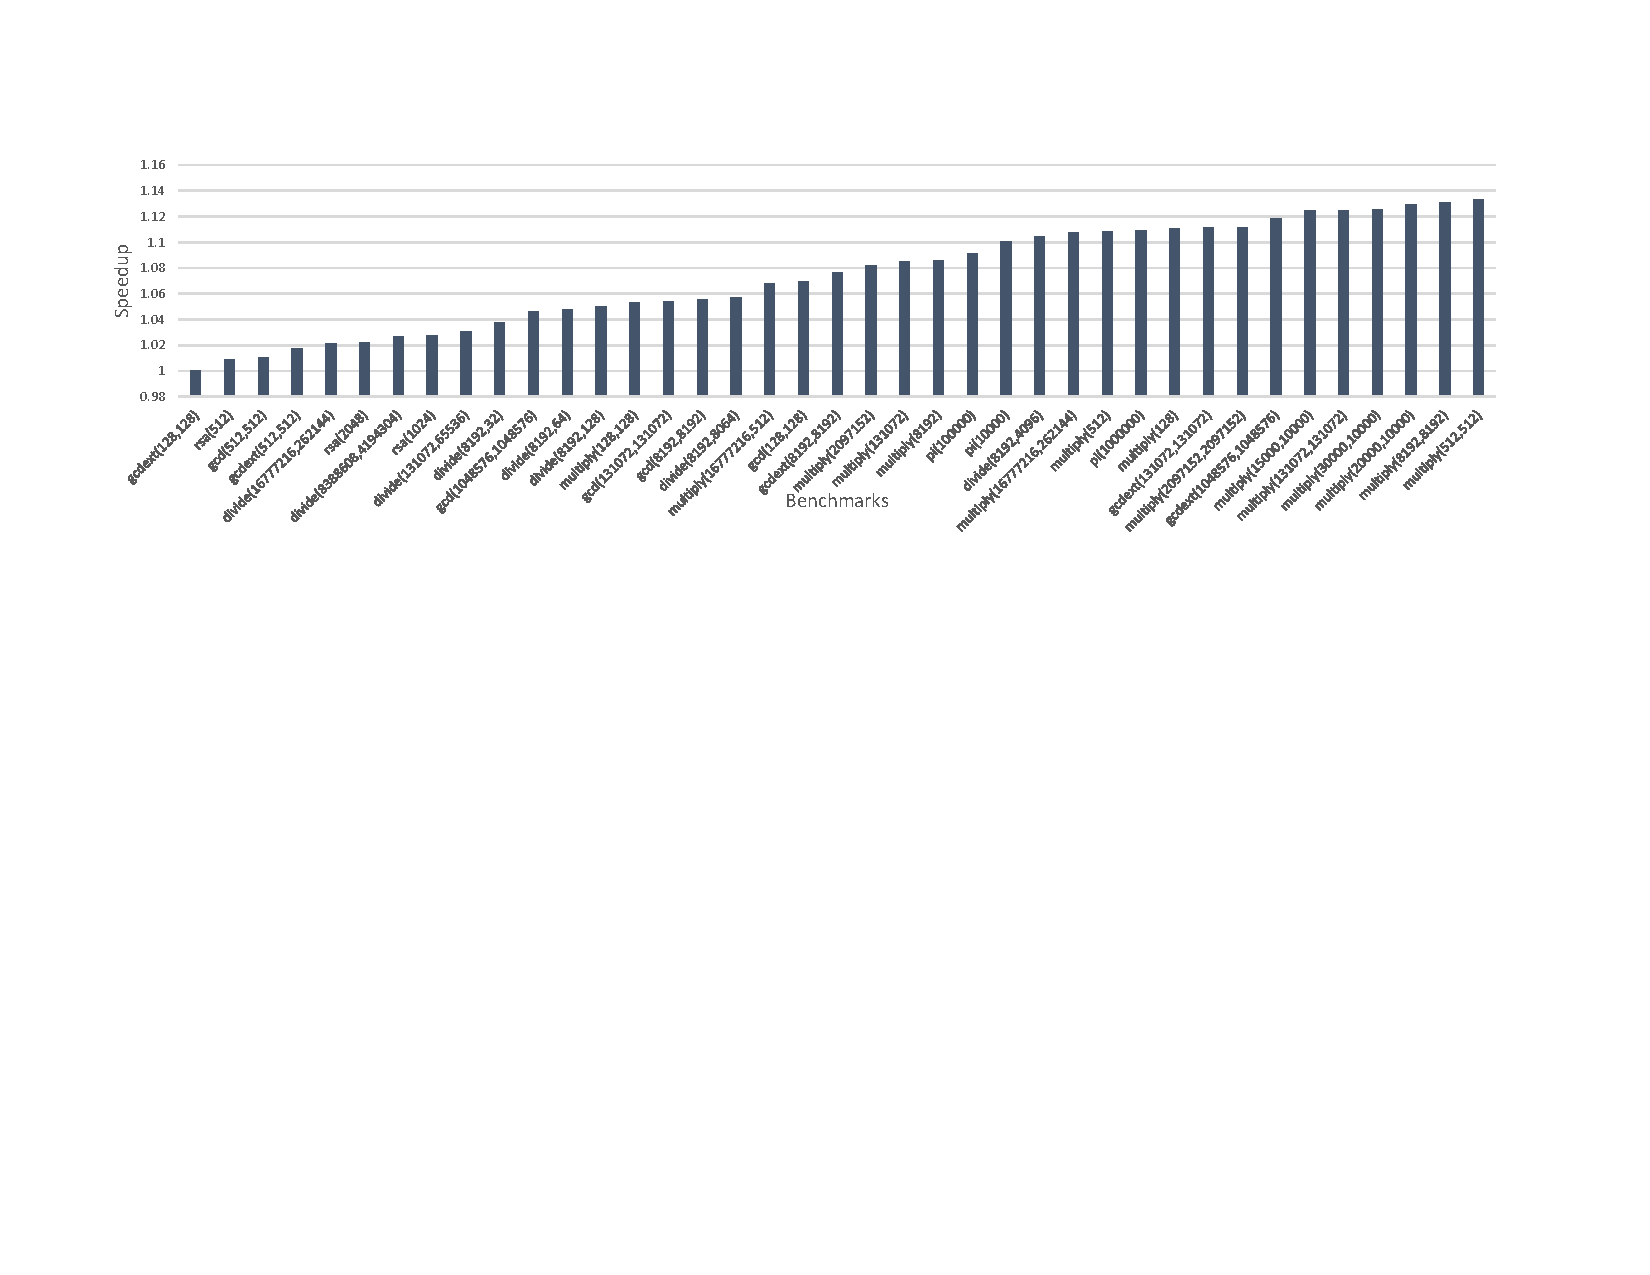
\includegraphics[page=1,width=\linewidth]{figures/data.pdf}
  }
  \hfill
  \subfloat[Speedups on AMD Zen 3, geomean = 1.065x\label{plot:gmp-amd}]{
    \includegraphics[page=2,width=\linewidth]{figures/data.pdf}
  }
  \caption{GNU Multiple Precision Library (GMP) speedups}
  \label{fig:gmp}
\end{figure}


GMP provides a portable C-language implementation and then, for
several platforms, a faster assembly language implementation.
%
For this evaluation, we selected the C implementation, because \minotaur{}
works on LLVM IR and cannot process assembly code at all.
%
The benchmark suite that we used is
GMPbench.%\footnote{\url{https://gmplib.org/gmpbench}}
%
Figure~\ref{fig:gmp} summarizes the results.
%
When \minotaur{} targets the Intel Cascade Lake processor, and when the
resulting executables are run on that same microarchitecture,
all the benchmarks sped up;
across all of the benchmarks, the mean speedup was 7.3\%.
%
The analogous experiment using the AMD Zen~3 microarchitecture
resulted in one benchmark slowing down, and the rest of benchmarks
speeding up, for an overall mean speedup of 6.5\%.


\paragraph{Optimizing libYUV with \minotaur{}}

\begin{figure}[tbp]
  \centering
  \subfloat[Speedups on Intel Cascade Lake, geomean = 1.022x\label{plot:libyuv-intel}]{
    \includegraphics[page=3,width=\linewidth]{figures/data.pdf}
  }
  \hfill
  \subfloat[Speedups on AMD Zen 3, geomean = 1.029x\label{plot:libyuv-amd}]{
    \includegraphics[page=4,width=\linewidth]{figures/data.pdf}
  }
  \caption{LibYUV speedups}
  \label{fig:yuv}
\end{figure}


This library has an extensive test suite, part of which is explicitly
intended for performance testing; we used this part as a benchmark.
%
Each of them scales, rotates, or converts a 1280\,x\,728 pixel
image 1,000 times.
%
Figure~\ref{fig:yuv} shows the results of this experiment.
%
When \minotaur{} targets an Intel processor, $148$ programs slowed down, $72$
did not change performance, and $2,312$ sped up, for an overall speedup of
2.2\%.
%
Targeting an AMD processor, $188$ programs slowed down, $85$ did not
change performance, and $2,259$ sped up, for an overall speedup of 2.9\%.
%
\minotaur{} can make code slower because it looks at optimizations in
isolation; it does not attempt to model interactions between
optimizations.


libYUV is portable code, but it has already been heavily tuned for
performance; most commits to its repository over the last several
years have been performance-related.
%
Our hypothesis is that this manual tuning has already eaten up most of
the performance gains that we would have hoped to gain from \minotaur{}.
%
For some time now, Google's released versions of Chrome have been
compiled using LLVM; the Chrome engineers have had ample time to
ensure that this compiler achieves decent code generation for
performance-critical libraries.

% \begin{figure*}[tbp]
%   \centering
%   \subfloat[Normalized speedup; geomean = 1.013x\label{fig:spec-intel-speed-ups}]{
%     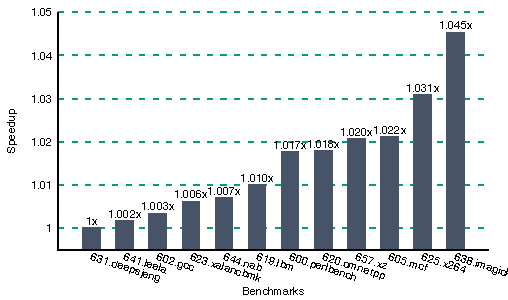
\includegraphics[width=0.45\linewidth]{figures/spec/spec-intel.pdf}
%   }
%   \hfill
%   \subfloat[Compilation time in seconds\label{fig:spec-intel-compilation-time}]{
%     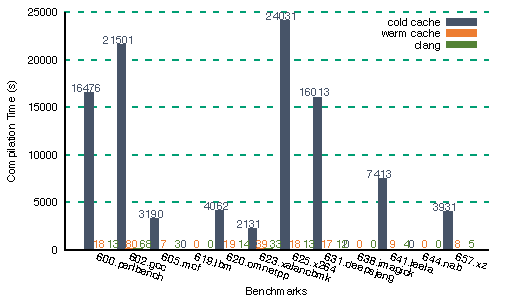
\includegraphics[width=0.45\linewidth]{figures/spec/spec-intel-compiletime.pdf}
%   }
%   \caption*{Targeting Intel Cascade Lake\label{fig:spec-intel}}
%   \hfill
%   \subfloat[Normalized speedup; geomean = 1.012x\label{fig:spec-amd-speed-ups}]{
%     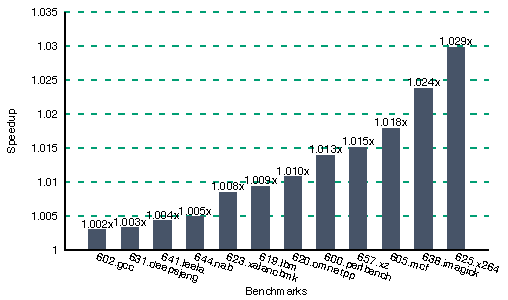
\includegraphics[width=0.45\linewidth]{figures/spec/spec-amd.pdf}
%   }
%   \hfill
%   \subfloat[Compilation time in seconds\label{fig:spec-amd-compilation-time}]{
%     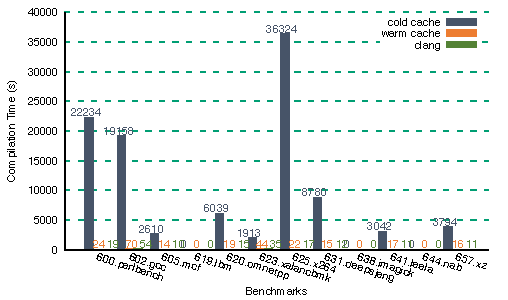
\includegraphics[width=0.45\linewidth]{figures/spec/spec-amd-compiletime.pdf}
%   }
%   \caption*{Targeting AMD Zen 3\label{fig:spec-amd}}
%   \caption{SPEC CPU2017 benchmark performance and compilation time}
%   \label{fig:spec}
% \end{figure*}

\begin{figure}[tbp]
  \centering
  \subfloat[Speedups on Cascade Lake; geomean = 1.015x\label{fig:spec-intel-speed-ups}]{
    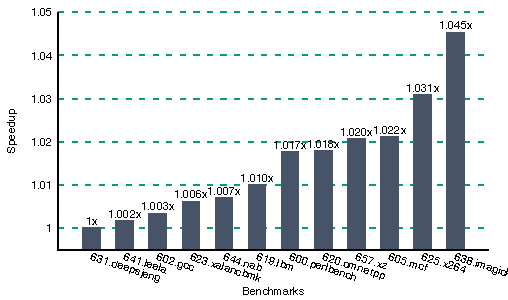
\includegraphics[width=0.48\linewidth]{figures/spec/spec-intel.pdf}
  }
  \hfill
  \subfloat[Speedups on Zen 3; geomean = 1.012x\label{fig:spec-amd-speed-ups}]{
    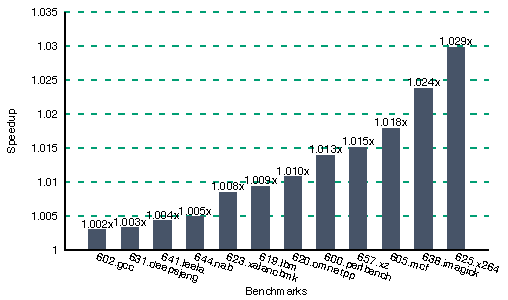
\includegraphics[width=0.48\linewidth]{figures/spec/spec-amd.pdf}
  }
  \caption{SPEC CPU2017 benchmark performance}
  \label{fig:spec}
\end{figure}

\paragraph{Optimizing SPEC CPU2017 with \minotaur{}}

Figure~\ref{fig:spec} shows the effect of optimizing the benchmarks
from SPEC CPU2017 using \minotaur.
%
When optimizing for, and running on, the Intel processor, we observed
a mean speedup of 1.5\%.
%
When optimizing for, and running on, the AMD processor, we observed a
mean speedup of 1.2\%.
%
It is notoriously difficult to speed up the SPEC CPU benchmarks
because compiler engineers have already put considerable effort into
achieving good code generation for them.



\subsection{Optimizations Discovered by \minotaur}
\label{sec:examples}

The purpose of this section is to examine \minotaur's strengths by
presenting some optimizations that it found while compiling benchmark
programs.
%
None of these optimizations can be performed by the version of LLVM
that \minotaur{} is based on,
%\footnote{\minotaur{} uses LLVM~18.1.0 for all results in this paper.}
at its \texttt{-O3} optimization level.
%
We present optimizations in an SSA format that is close to LLVM IR,
but we have edited it slightly for compactness and legibility.

\iffalse
One might be inclined to ask, while reading this section, ``Why is
LLVM incapable of performing this transformation?''
%
Alas, there is no single answer.
%
In some cases, performing the transformation would require the
optimizer to have a semantic model of a processor-specific intrinsic
function, but mostly these models do not exist.
%
In other cases, such as Example~5 below, generic reasoning about the
code would be very difficult, and a specific pattern matcher might not
be robust enough to be worth implementing.
%
Finally, our observation is that vector support in LLVM is somewhat
newer and less mature than support for other IR features, and the
optimizers have simply not had enough time to accumulate the requisite
optimizations.
\fi


\paragraph*{Example 1}

This code is from perlbench in SPEC:

{\begin{quote}\begin{verbatim}
%0 = zext <16 x i8> %x to <16 x i16>
%1 = zext <16 x i8> %y to <16 x i16>
%2 = call @llvm.x86.avx2.pavg.w(%0, %1)
%3 = trunc <16 x i16> %2 to <16 x i8>
ret <16 x i8> %3
  =>
%0 = call @llvm.x86.sse2.pavg.b(%x, %y)
ret <16 x i8> %0
\end{verbatim}
\end{quote}}

The unoptimized code zero-extends each 8-bit element of the two input
vectors to 16~bits, calls the AVX2 variant of \texttt{pavg} to perform
element-wise averaging of the extended vectors, and then truncates
elements of the resulting vector back to eight bits.
%
The optimized code simply calls an SSE2 version of the \texttt{pavg}
instruction that operates on 8-bit elements, reducing the uOp cost
of the operation from four to one.


\paragraph*{Example 2}
%https://godbolt.org/z/vjjr7MGzb

This code is from libYUV, ``... an open source project that includes
YUV scaling and conversion
functionality'':
%m\footnote{\url{https://chromium.googlesource.com/libyuv/libyuv/}}

{\begin{quote}\begin{verbatim}
%0 = call @llvm.x86.avx2.pmadd.wd(%x, <0,1,0,1, ...>)
%1 = call @llvm.x86.avx2.pmadd.wd(%x, <1,0,1,0, ...>)
%2 = sub nsw <8 x i32> %1, %0
ret <8 x i32> %2
  =>
%0 = call @llvm.x86.avx2.pmadd.wd(%x,<1,-1,1,-1, ...>)
ret <8 x i32> %0
\end{verbatim}
\end{quote}}

The \texttt{pmadd.wd} (multiply and add packed integers) instruction multiplies
signed 16-bit integers element-wise from two input vectors, and then
computes its output by adding adjacent pairs of elements from the
resulting vector.
%
Thus, the input to this instruction is two 16-way vectors containing
16-bit elements, and its output is a single 8-way vector of 32-bit
elements.


In this example, the second argument to each \texttt{pmadd.wd}
instruction in the unoptimized code is a vector of alternating zeroes
and ones, which has the effect of selecting odd-indexed elements into
\texttt{\%0} and even-indexed elements into \texttt{\%1}.
%
Then, after the \texttt{sub} instruction, which simply performs
element-wise subtraction of \texttt{\%0} and \texttt{\%1}, the overall
effect of this code is to compute the difference between adjacent
pairs of elements of \texttt{\%x}.
%
\minotaur{} is able to perform this same computation using a single
\texttt{pmadd.wd} instruction which negates odd-numbered elements of
\texttt{\%x} before performing the addition.
%
The optimized code requires $5$ uOps to execute whereas the original
code requires $8$.


\paragraph*{Example 3}

This code is from libYUV:

%https://godbolt.org/z/7ooobqofK
{\begin{quote}\begin{verbatim}
%0 = shufflevector <32 x i8> %x, poison, <3, 7, 11, 15, 19, 23, 27, 31>
%1 = lshr %0, <6, 6, 6, 6, 6, 6, 6, 6>
%2 = zext 8 x i8> %1 to <8 x i32>
ret <8 x i32> %2
  =>
%0 = bitcast <32 x i8> %x to <8 x i32>
%1 = call @llvm.x86.avx2.psrli.d(<8 x i32> %0, 30)
ret <8 x i32> %1
\end{verbatim}
\end{quote}}

The \texttt{shufflevector} instruction in the unoptimized code selects
every fourth byte-sized element from the input \texttt{\%x}.
%
The resulting 8-way vector is right-shifted element-wise by six bit
positions, and that result is zero-extended to an 8-way vector of
32-bit elements.
%
\minotaur's optimized version (which executes in 4 uOps instead of 11)
first reinterprets the input vector's data as 32-bit elements; this
bitcast is relevant to LLVM's type system, but it is a nop at the CPU
level.
%
Then, the \texttt{prsli} instruction shifts each 32-bit element to the
right by 30 bit positions.
%
This right-shift-by-30 achieves the same effect as the unoptimized
code, where the \texttt{shufflevector} can be seen as a
right-shift-by-24, followed by an explicit right-shift-by-6.

\paragraph*{Example 4}

This code, from compiling perlbench from SPEC CPU 2017, illustrates
\minotaur's ability to reason about control flow:

% control flow divergence
%https://godbolt.org/z/e8jTsTMMz
{\begin{quote}\begin{verbatim}
entry:
  br i1 %c, label %body, label %if.end
body:
  br label %if.end
if.end:
  %p1 = phi [ %a, %body ], [ %b, %entry ]
  %p2 = phi [ %b, %body ], [ %a, %entry ]
  %r = call @llvm.x86.avx2.pavg.b(%p1, %p2)
  ret <32 x i8> %r
    =>
  %r = call @llvm.x86.avx2.pavg.b(%a, %b)
  ret <32 x i8> %r
\end{verbatim}
\end{quote}}

The intent of the code is to compute the element-wise average of input
vectors \texttt{\%a} and \texttt{\%b}, with a Boolean value
\texttt{\%c} determining the order in which the input vectors are
presented to the \texttt{pavg} instruction.
%
However, the order of arguments to this instruction does not matter, and
\minotaur's version executes in 4 uOps while the original code requires
10.
%
Note that \minotaur{} was not explicitly taught that \texttt{pavg} is
commutative; the necessary information was inferred naturally from the
formal specification.


\paragraph*{Example 5}

This is an optimization discovered
by \minotaur{} when it was used to compile GMP, the GNU Multiple Precision
Arithmetic Library, a widely-used library for arbitrary precision
integer computation:
%q\footnote{\url{https://gmplib.org/}}

% before 19 after 13

{\begin{quote}\begin{verbatim}
%0 = lshr i64 %x, 1
%1 = and i64 %0, 0x5555555555555555
%2 = sub i64 %x, %1
%3 = lshr i64 %2, 2
%4 = and i64 %2, 0x3333333333333333
%5 = and i64 %3, 0x3333333333333333
%6 = add nuw nsw i64 %4, %3
%7 = lshr i64 %6, 4
%8 = add nuw nsw i64 %7, %6
%9 = and i64 %8, 0xf0f0f0f0f0f0f0f
ret i64 %9
  =>
%0 = bitcast i64 %x to <8 x i8>
%1 = call @llvm.ctpop(<8 x i8> %0)
%2 = bitcast <8 x i8> %1 to i64
ret i64 %2
\end{verbatim}
\end{quote}}

%
% \vspace{0.1in}
% %
% \caption{On the left, LLVM IR extracted from GMP; when compiled to
%   x86-64 code and run on an Intel Cascade Lake processor, its
%   predicted execution cost is 19 uOps. On the right, \minotaur's
%   optimized version of this code, which requires 13 uOps on the same
%   target.}
% \label{fig:ctpop}
% \end{figure*}
%
The original code performs a series of bit-level
manipulations on a 64-bit integer value, with the net result of
performing an 8-way vectorized 8-bit popcount operation.\footnote{The
popcount, or Hamming weight, of a bitvector is the number of ``1''
bits in it.}
%
The optimized code simply calls an intrinsic function to do the
popcount; it costs 13 uOps instead of the original code's 19.
%
Although robust recognition of open-coded idioms is not the focus
of our work, \minotaur{} does sometimes manage to achieve this.

Taking a strict view of types in the synthesis process could help
prune the search space, but it would also cause us to miss
optimizations that require a flexible view of types.
%
This example illustrates the latter case: the original code contains
no indication that a good optimization can be found using a vector of
type <8 x i8>, and therefore a strictly type-guided synthesis
procedure would miss this one.

\paragraph*{Example 6}

This code comes from 644.nab in SPEC CPU 2017:

% https://github.com/llvm/llvm-project/issues/85250
{\begin{quote}\begin{verbatim}
%0 = fcmp oge float %x, 0.000000e+00
%1 = fneg float %x
%2 = select i1 %0, float %0, float %2
%3 = fcmp oeq float %2, 0.000000e+00
ret i1 %3
  =>
%1 = fcmp oeq float %x, 0.000000e+00
ret i1 %oeq
\end{verbatim}
\end{quote}}

The original code computes the absolute value of a floating-point
number \texttt{\%x} and then checks if the result is zero.
\minotaur{} found that that the original code is equivalent to simply checking if
\texttt{\%x} is zero.


\paragraph*{Example 7}

This code is from the SPEC CPU 2017 benchmark 619.lbm:

% https://github.com/llvm/llvm-project/issues/85245
{\begin{quote}\begin{verbatim}
%0 = fsub float %x, %y
%1 = fcmp ogt float %0, 0.000000e+00
ret i1 %3
  =>
%0 = fcmp ogt float %x, %y
ret i1 %0
\end{verbatim}
\end{quote}}

The original code computes the difference between two floating-point
values, and then checks if the result is greater than zero. \minotaur{}
found that this code is equivalent to checking if the second value is
less than the first.


\paragraph*{Example 8}

This code comes from 619.lbm in SPEC CPU 2017:

% https://github.com/llvm/llvm-project/issues/85267

{\begin{quote}\begin{verbatim}
%0 = fmul float %x, 0x3FF0CCCCC0000000
%1 = fcmp olt float %t1, 0x3FE20418A0000000
ret i1 %1
  =>
%0 = fcmp ole float %x, 0x3FE12878E0000000
ret i1 %0
\end{verbatim}
\end{quote}}

The original code multiplies a floating-point value \texttt{\%x} by a
constant, and then checks if the result is less than another constant.
\minotaur{} found that this code is equivalent to checking if \texttt{\%x}
is less than or equal to a third constant.
It is tricky to reason about floating-point literals, and \minotaur{} is able to
reason and synthesize the correct literals correctly.

\paragraph*{Example 9}

This code comes from 638.imagick in SPEC CPU 2017:

{\begin{quote}\begin{verbatim}
%0 = fmul float %x, 0.000000e+00
%1 = fmul float %0, 3.000000e+00
ret float %1
  =>
%0 = fmul float %x, 0.000000e+00
ret i1 %0
\end{verbatim}
\end{quote}}

The original code multiplies a floating-point value \texttt{\%x} by
zero, and then multiplies the result by 3.0. \minotaur{} found that this
code is equivalent to multiplying \texttt{\%x} by zero directly.
Note the original code cannot be optimized to 0.0 directly, because of
the NaN and signed zero propagation rules in floating-point arithmetic.
This example shows that \minotaur{} is able to reason about these corner
cases and synthesize the correct code.

% \paragraph*{Example 10}


%TODO: Add one final example
% place holder for a good example




